\documentclass{beamer}
\mode<presentation>
{
  \usetheme{default}
  \usecolortheme{default}
  \usefonttheme{default}
  \setbeamertemplate{navigation symbols}{}
  \setbeamertemplate{caption}[numbered]
}
\addtobeamertemplate{navigation symbols}{}{
    \usebeamerfont{footline}
    \usebeamercolor[fg]{footline}
    \hspace{1em}
    \insertframenumber/\inserttotalframenumber
}
\usepackage{array}
\usepackage{xcolor}
\usepackage{hyperref}
\usepackage[english]{babel}
\usepackage[utf8x]{inputenc}
\DeclareMathOperator*{\argmax}{arg\,max}
\DeclareMathOperator*{\argmin}{arg\,min}
\title[IEEE ICC 2021]{\small{\textcolor{black}{IEEE ComSoc ICC 2021 CRAIN Symposium}}\\\Large{Learning-based Cognitive Radio Access via Randomized Point-Based Approximate POMDPs}}
\author{Bharath Keshavamurthy\textsuperscript{*}, IEEE Student Member\\
Nicol\`{o} Michelusi\textsuperscript{\#}, IEEE Senior Member}
\institute{\textsuperscript{*}PhD Student, School of Electrical and Computer Engineering, Purdue University\\
\textsuperscript{\#}Assistant Professor, School of Electrical, Computer and Energy Engineering, Arizona State University}
\date{}
\begin{document}
\begin{frame}
  \titlepage
\end{frame}
\begin{frame}{Motivation (1/2)}
\begin{figure}
    \centering
    \footnote{\tiny{Drew Fitzgerald, The Wall Street Journal, Dec 28, 2019}}
    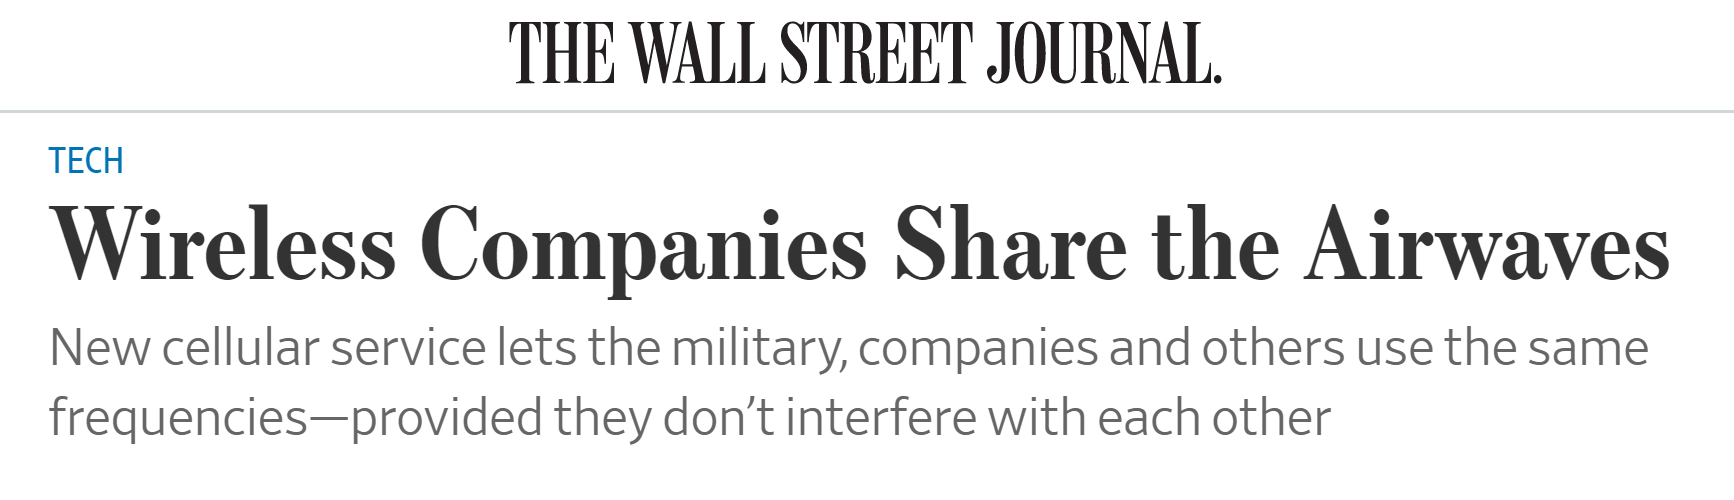
\includegraphics[width = 0.8\textwidth]{figs/WSJ_1.PNG}
    \label{fig:1a}
\end{figure}
\begin{figure}
    \centering
    \footnote{\tiny{WSJ Opinion Letters, The Wall Street Journal, Feb 7, 2020}}
    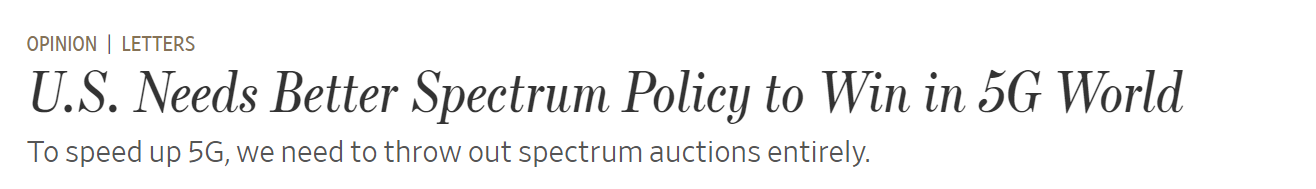
\includegraphics[width = 0.8\textwidth]{figs/WSJ_2_mod.PNG}
    \label{fig:1b}
\end{figure}
\begin{figure}
    \centering
    \footnote{\tiny{Holman W. Jenkins Jr, The Wall Street Journal, June 14, 2019}}
    
\includegraphics[width = 0.8\textwidth]{figs/WSJ_3_mod.PNG}
    \label{fig:1c}
\end{figure}
\end{frame}
\begin{frame}{Motivation (2/2)}
\begin{figure}
    \centering
    \footnote{\tiny{5G Use Cases, Ericsson, [\href{https://www.ericsson.com/assets/local/news/2015/7/5g-use-cases.pdf}{\textcolor{blue}{Online}}] Nov 26, 2015}}
    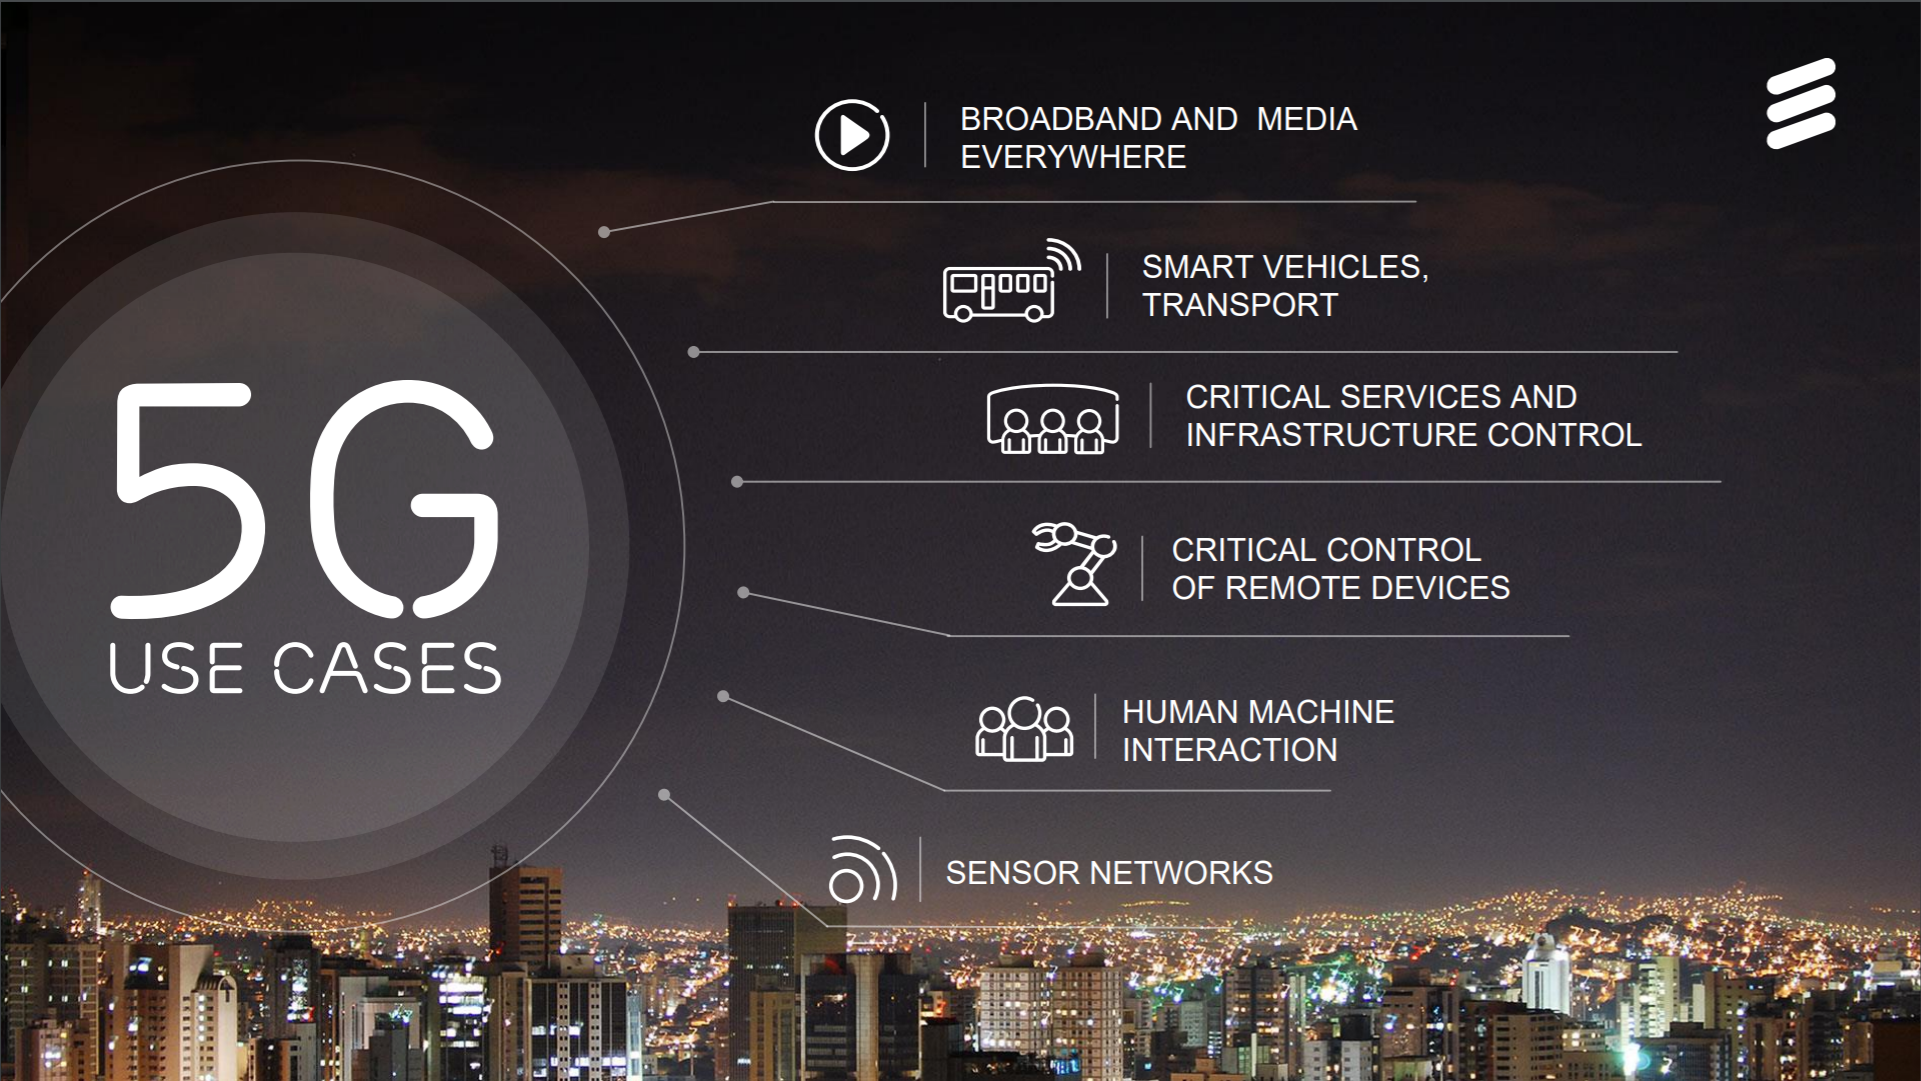
\includegraphics[width = 0.6\textwidth]{figs/Ericsson.PNG}
    \label{fig:1d}
\end{figure}
\begin{figure}
    \centering
    \footnote{\tiny{Alison Gopnik, The Wall Street Journal, Oct 11, 2019}}
    
\includegraphics[width = 0.6\textwidth]{figs/WSJ_4.PNG}
    \label{fig:1e}
\end{figure}
\end{frame}
\begin{frame}{Problem Description\footnote{\tiny{Primary Users (PUs) are the licensed users/incumbents $|$ Secondary Users (SUs) are the cognitive radio nodes}}}
\begin{figure}
    \centering
    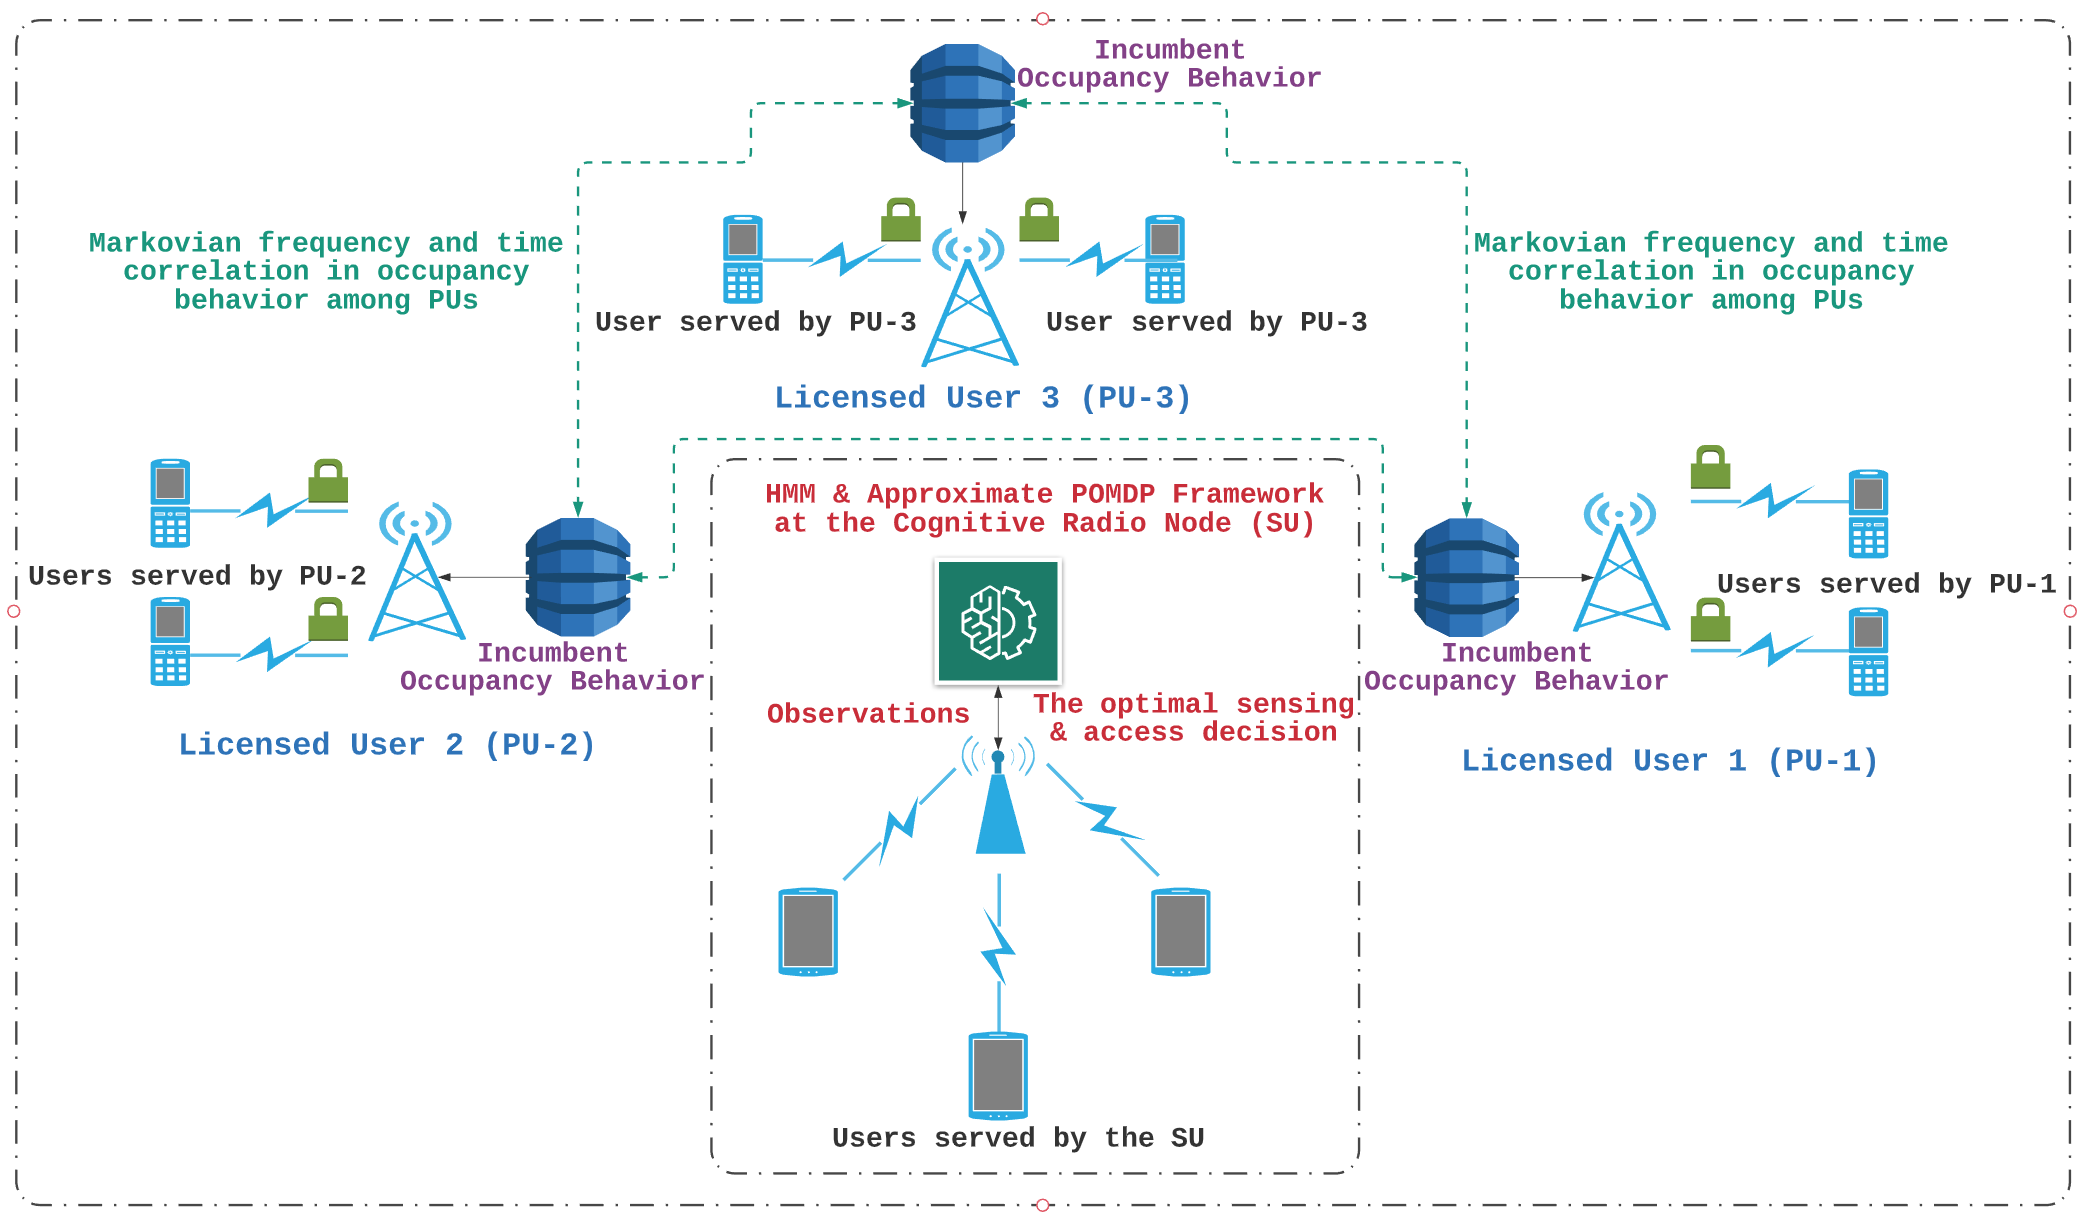
\includegraphics[width = 0.95\textwidth]{figs/System_Model_1.png}
    \caption{An \textcolor{magenta}{example of a heterogeneous radio ecosystem} in which cognitive radio technology is a game-changer}
    \label{fig:1f}
\end{figure}
\end{frame}
\begin{frame}{Challenges}
    \begin{itemize}
        \footnotesize{
        \item \textcolor{blue}{Noisy observations at the SU receiver} hide the true occupancy states of the channels -- impairing accurate white-space detection \& access\footnote{\tiny{F. Xu, et. al., ``Architecture for Re-configurable Networks via Cognitive Radio", 2008 CROWNCOM}}
        \item \textcolor{blue}{Energy efficiency needs at the SU} constrain the number of channels that it can sense in a time-slot\footnote{\tiny{S. Malecki, et. al., ``Energy and throughput efficient strategies for spectrum sensing...", 2011 IEEE SPAWC}}
        \item \textcolor{blue}{Occupancy behaviors of PUs are correlated} across time AND frequency\footnote{\tiny{Active Incumbent, DARPA SC$2$, [\href{https://sc2colosseum.freshdesk.com/support/solutions/articles/22000239489-active-incumbent-}{\textcolor{blue}{Online}}], Aug 28, 2019}}
        \item This time-frequency \textcolor{blue}{correlation model is not known a priori}
        \item The capability to \textcolor{blue}{regulate the trade-off between SU and PU(s) throughputs} is crucial
        \item \textcolor{blue}{The curse of dimensionality}}
    \end{itemize}
\end{frame}
\begin{frame}{Related Work $|$ State-of-the-Art (SoA)}
Custom heuristics\footnote{\label{F4}\tiny{M. Gao, et. al., ``Fast Spectrum Sensing...", 2014 IEEE MilCom}} $|$ Hidden Markov Models (HMMs)\footnote{\label{F6}\tiny{C. Park, et. al., ``HMM Based Channel Status Predictor for Cognitive Radio", 2007 APAC MW Conference}}\\Multi-Armed Bandits (MABs)\footnote{\label{F5}\tiny{K. Cohen, et. al., ``Restless Multi-Armed Bandits...", 2014 Asilomar}} $|$ Reinforcement Learning (RL)\footnote{\label{F3}\tiny{J. Lund\'{e}n, et. al., ``Multiagent Reinforcement Learning...", IEEE Journal of Selected Topics in SigProc, 2013}}
\footnotesize{
\begin{center}
    \begin{tabular}{ || c | c || }
        \hline
        \textcolor{blue}{Drawbacks in SoA} & \textcolor{blue}{Our Answers}\\
    	\hline\hline
    	\textcolor{red!75!blue}{Noise-free} [\ref{F4}] obs \& \textcolor{red!75!blue}{Ignored} [\ref{F3}] est errors & \textcolor{green!65!blue}{Noisy} obs $|$ \textcolor{green!65!blue}{HMMs}\\
    	\hline
    	\textcolor{red!75!blue}{Failure to exploit} [\ref{F5}] PU correlation & \textcolor{green!65!blue}{Successful exploitation}\\
    	\hline
    	\textcolor{red!75!blue}{Apriori knowledge} [\ref{F3}] & \textcolor{green!65!blue}{No apriori knowledge}\\
    	\hline
    	\textcolor{red!75!blue}{Offline estimation} [\ref{F4}] & \textcolor{green!65!blue}{Fully Online estimation}\\
    	\hline
    	\textcolor{red!75!blue}{No support} [\ref{F4}], [\ref{F3}] for tuning throughputs & \textcolor{green!65!blue}{Support} via penalty tuning\\
    	\hline
    \end{tabular}
\end{center}}
Our framework is evaluated against [\ref{F4}], [\ref{F6}], and [\ref{F3}] (among others -- including \textcolor{blue}{Deep-Q Networks (DQNs)}, the \textcolor{blue}{Viterbi Algorithm}, and \textcolor{blue}{Neyman-Pearson Detection}): \textcolor{green!65!blue}{We demonstrate superior performance}.
\end{frame}
\begin{frame}{System Model}
\footnotesize{\textcolor{magenta}{OFDMA}; \textcolor{magenta}{AWGN} observation model; \textcolor{magenta}{Rayleigh} fading channel; \textcolor{magenta}{Sensing limits}}
\begin{figure}
    \centering
    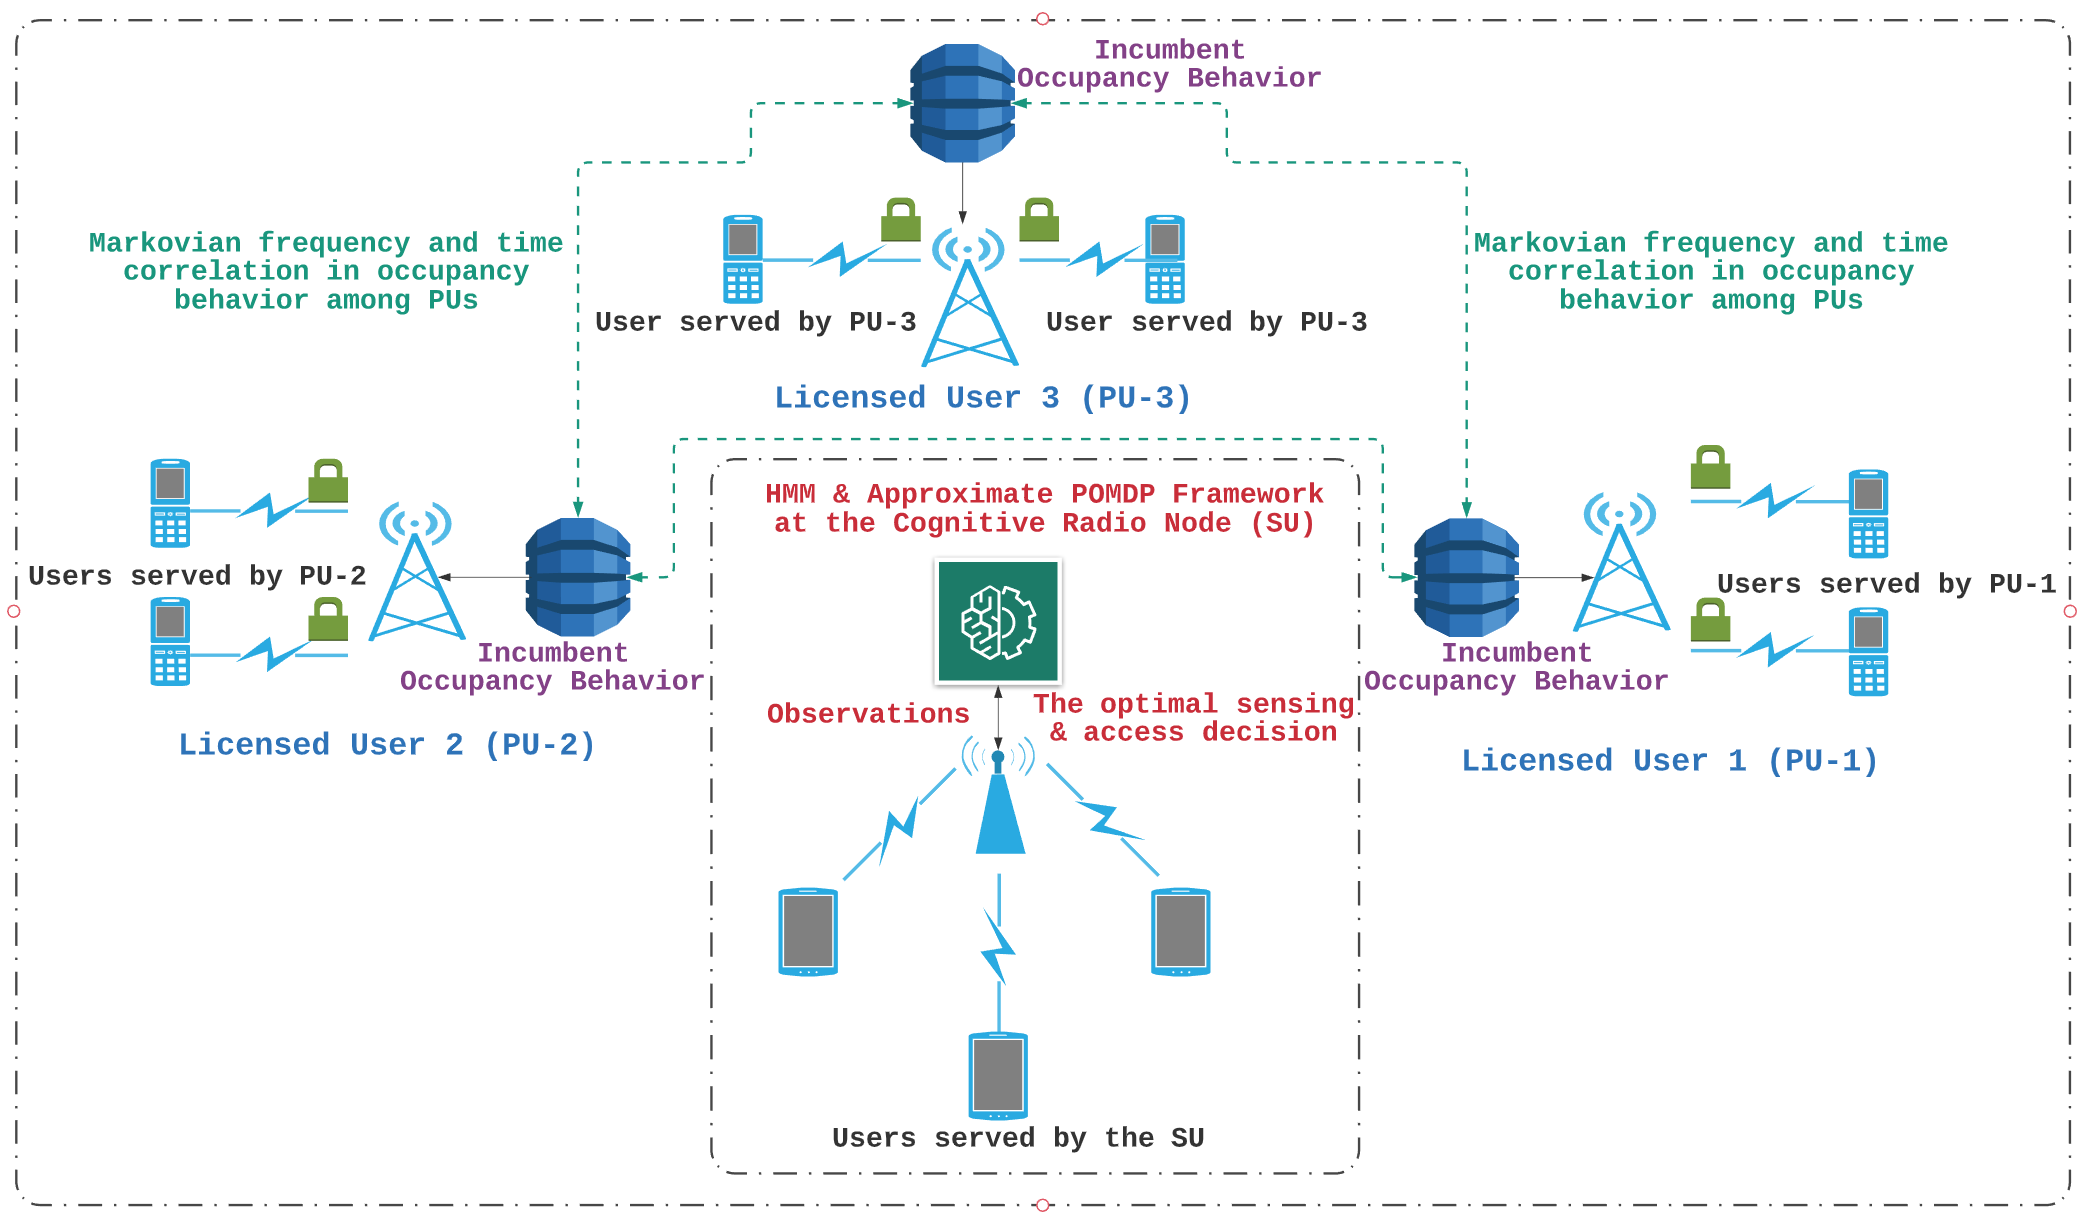
\includegraphics[width = 1.0\textwidth]{figs/System_Model_1.png}
    \caption{An \textcolor{magenta}{exemplification of the radio ecosystem} under analysis:\newline $18$ channels, $3$ PUs, and $1$ SU with sensing limit - $3$ channels per time-slot}
    \label{fig:2a}
\end{figure}
\end{frame}
\begin{frame}{PU Occupancy Model\footnote{\tiny{Active Incumbent, DARPA SC$2$, [\href{https://sc2colosseum.freshdesk.com/support/solutions/articles/22000239489-active-incumbent-}{\textcolor{blue}{Online}}], Aug 28, 2019}}}
\footnotesize{\[\mathbb{P}(\vec{B}(i+1)|\vec{B}(i))=\mathbb{P}(B_{1}(i+1)|B_{1}(i))\prod_{k=2}^{K}\mathbb{P}(B_{k}(i+1)|B_{k}(i), B_{k-1}(i+1))\]}
\begin{figure}
    \centering
    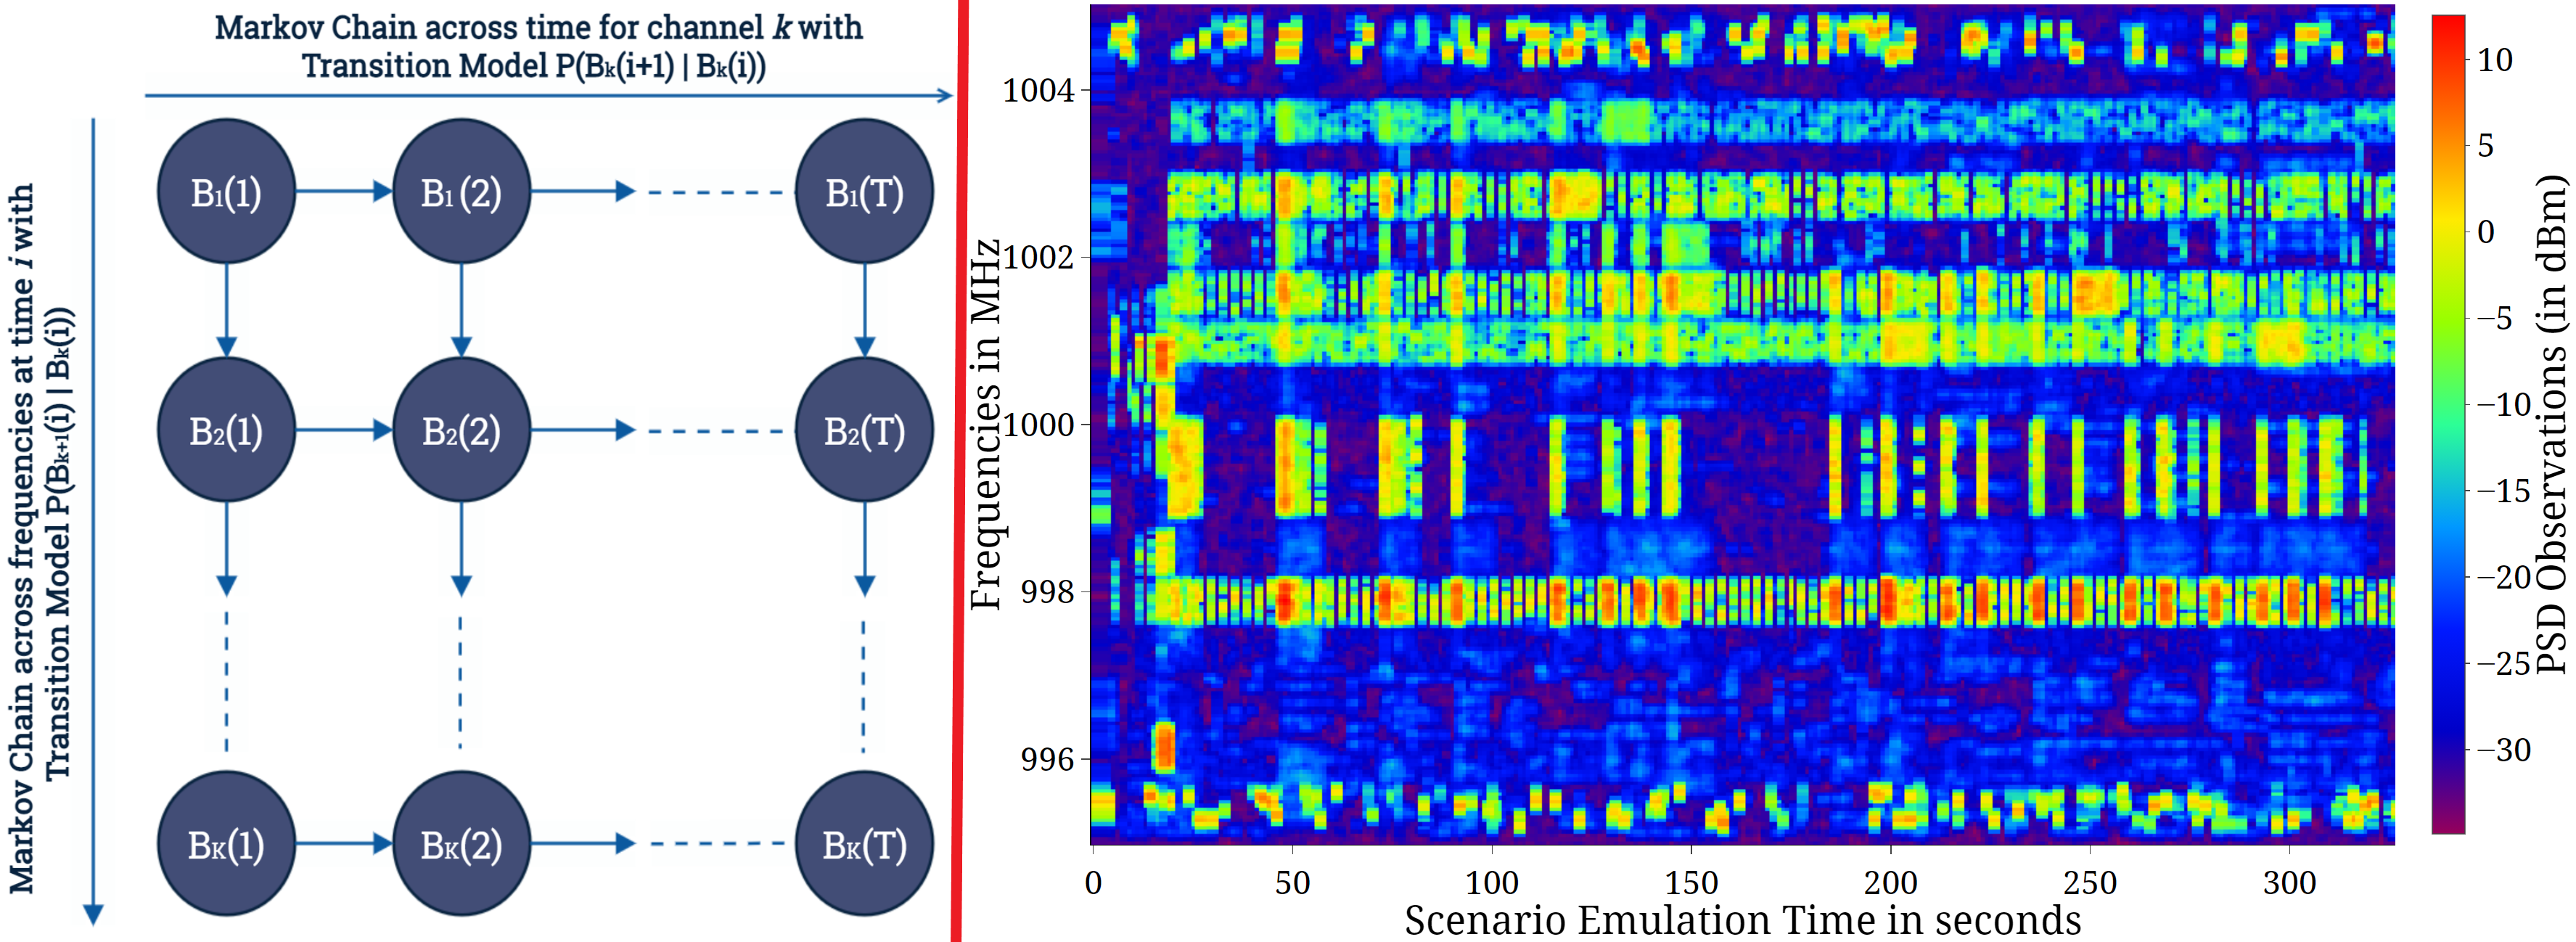
\includegraphics[width = 1.0\textwidth]{figs/Minerva_Markov_Chain_with_Aggregated_PSD_Observations.png}
    \caption{\textcolor{magenta}{Markovian time-frequency correlation} of PU occupancies $|$ Model Validation through DARPA SC$2$ Active Incumbent}
    \label{fig:2b}
\end{figure}
\end{frame}
\begin{frame}{SU Spectrum Sensing Model}
    \begin{itemize}
        \item SU can sense \textcolor{magenta}{at most $\kappa$ out of $K$ spectrum bands at any given time}, with $1{\leq}\kappa{\leq}K$
        \item HMM framework:
        \[\vec{Y}(i) = [Y_k(i)]_{k {\in} \mathcal K_i}\text{ is the observation vector}\]
        \[f(\vec{Y}(i)|\vec{B}(i), \mathcal K_i) = \prod_{k \in \mathcal K_i} f(Y_k(i)|B_k(i))\text{ is its PDF}\]
        \[Y_k(i)|B_k(i) \sim \mathcal{CN}(0, \sigma_H^2P_{tx}B_k(i) + \sigma_V^2)\]
    \end{itemize}
\end{frame}
\begin{frame}{POMDP Agent Model (1/2)}
   \begin{figure}
    \centering
    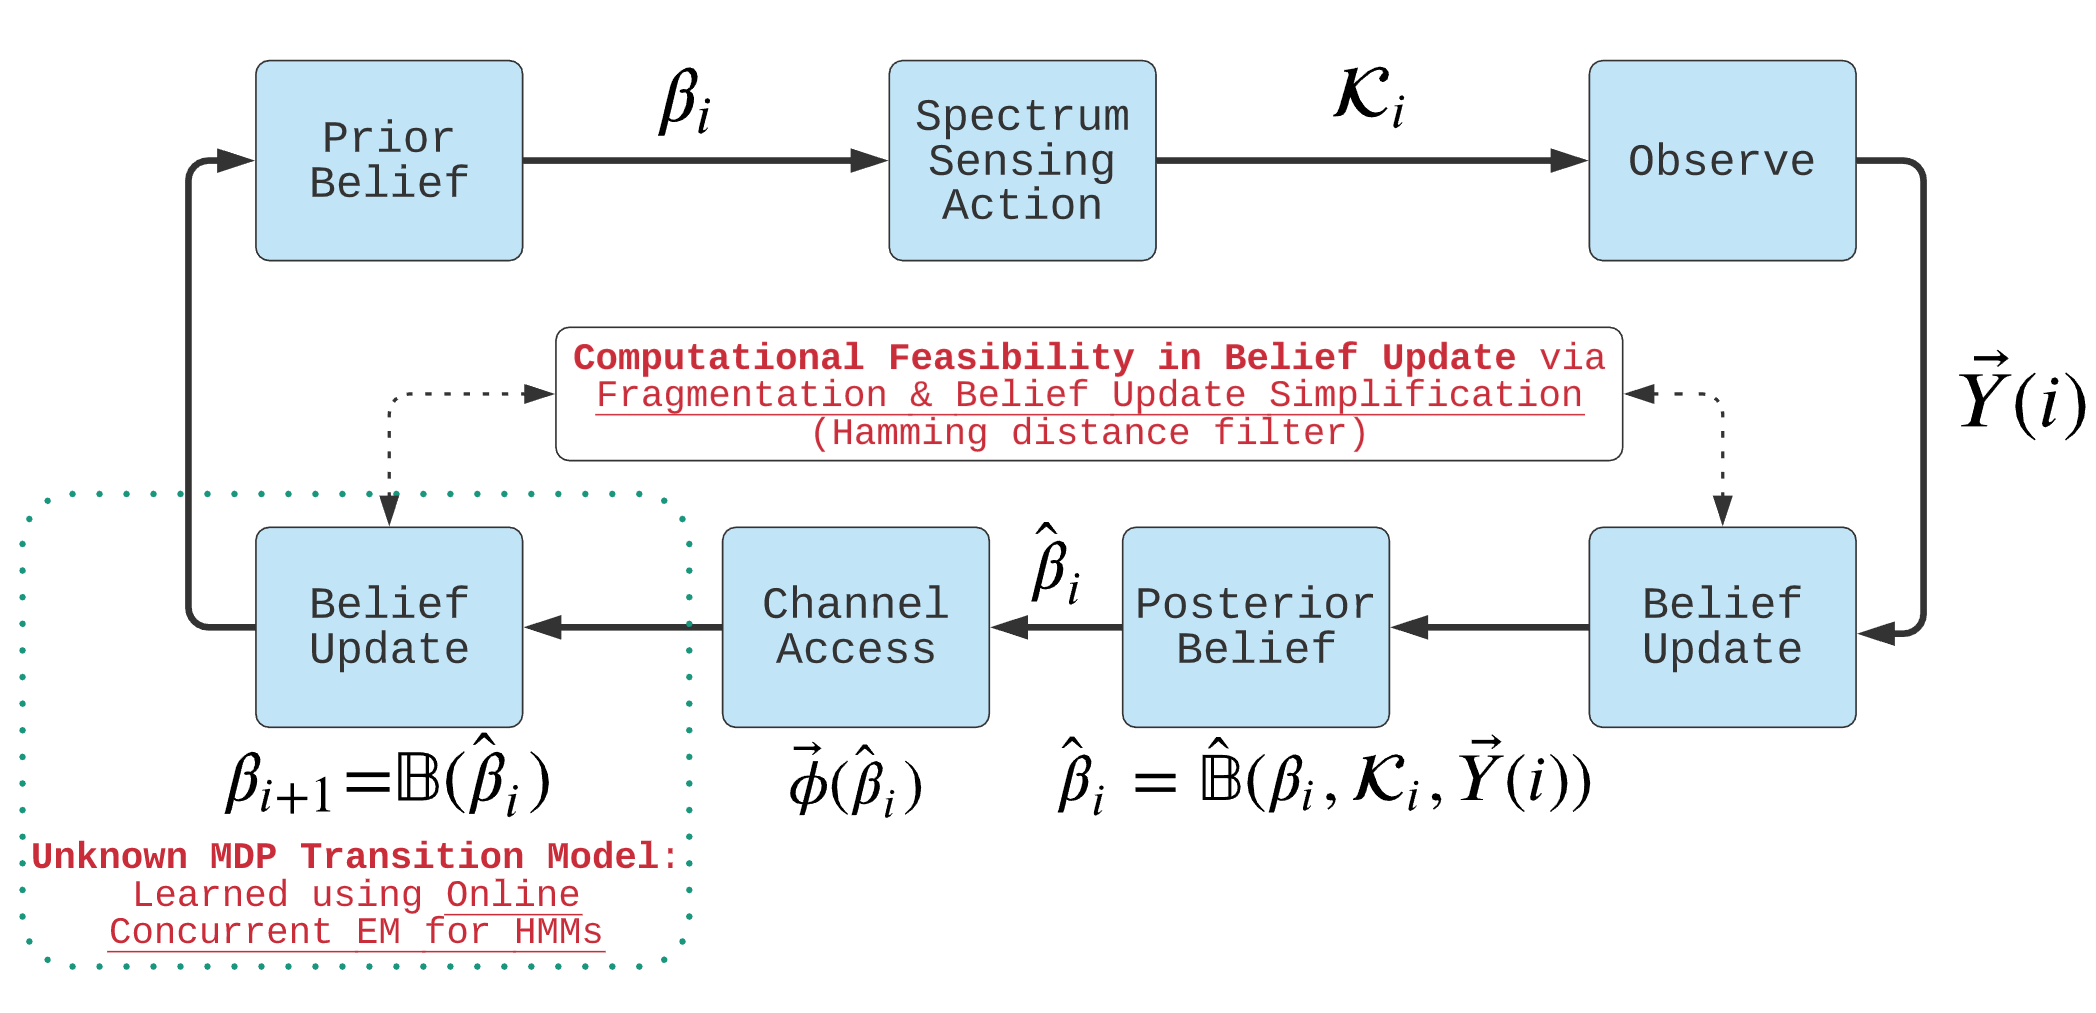
\includegraphics[width = 1.0\textwidth]{figs/Minerva_POMDP_Model.png}
    \caption{The POMDP Formulation}
    \label{fig:2c}
\end{figure}
\end{frame}
\begin{frame}{POMDP Agent Model (2/2)}
    \footnotesize{\begin{itemize}
        \item \textcolor{magenta}{Goal}: Find optimal spectrum sensing policy that maximizes the infinite-horizon discounted reward:
        \[\pi^{*}{=}\argmax_{\pi} V^{\pi}(\beta) \triangleq \mathbb{E}_{\pi} \Big[\sum_{i=1}^{\infty} \gamma^{i} R(\vec{B}(i), \hat{\beta}_i)|\beta_0 {=}\beta\Big]\]
        \item \textcolor{magenta}{Access decision}:
        \[\vec{\phi}(\hat{\beta}_{i})\triangleq \argmax_{\vec{B} {\in} \mathcal{B}} \hat{\beta}_{i}(\vec{B})\]
        \item \textcolor{magenta}{Reward formulation}:
        \[R(\vec{B}(i), \hat{\beta}_i){=}\sum_{k=1}^{K} (1{-}B_k(i))(1{-}\phi_k(\hat{\beta}_{i})){-}\lambda B_k(i)(1 - \phi_k(\hat{\beta}_i))\]
        \item $\pi^{*}$ is the solution to $V^*{=}\mathcal{H}[V^*]$; \textcolor{magenta}{Bellman operator} $V_{t+1}{=}\mathcal {H}[V_{t}]$ is ${\forall}\beta:$
        \[V_{t+1}(\beta) = \max_{\mathcal{K} {\in} \mathcal{A}} \sum_{\vec{B} {\in} \mathcal{B}} \beta(\vec{B}) \mathbb{E}_{\vec{Y}|\vec{B}, \mathcal{K}} \Big[R(\vec{B}, \hat{\mathbb{B}}(\beta, \mathcal{K}, \vec{Y}))+\gamma V_{t}(\mathbb{B}(\hat{\mathbb{B}}(\beta, \mathcal{K}, \vec{Y})))\Big]\]
    \end{itemize}}
\end{frame}
\begin{frame}{The Parameter Estimator\footnote{\tiny{L. Rabiner, ``A Tutorial on Hidden Markov Models and Selected Applications in Speech Recognition", Proceedings of the IEEE 77, no. 2, Feb 1989}}}
    \begin{itemize}
        \item \textcolor{magenta}{Goal}: Determine the time-frequency occupancy correlation structure of the PUs -- \textcolor{blue}{parameterized by $\vec{\theta}$}
        \item \textcolor{magenta}{Maximum Likelihood Estimation (MLE) problem}:
        \[\vec{\theta}^{*} = \argmax_{\vec{\theta}} \log\Big(\sum_{\mathbf{B}} \mathbb{P}(\mathbf{B}, \mathbf{Y}| \vec{\theta})\Big)\]
        \item \textcolor{magenta}{Baum-Welch} (Expectation-Maximization (EM) for HMMs):
        \[\text{\textcolor{magenta}{E-step}: }Q(\vec{\theta}|\vec{\theta}^{(t)}) = \mathbb{E}_{\mathbf{B}|\mathbf{Y}, \vec{\theta}^{(t)}} \Big[ \log \Big(\mathbb{P}(\mathbf{B}, \mathbf{Y}|\vec{\theta}^{(t)})\Big)\Big]\]
        \[\text{\textcolor{magenta}{M-step}: }\vec{\theta}^{(t+1)} = \argmax_{\vec{\theta}} Q(\vec{\theta}|\vec{\theta}^{(t)})\]
    \end{itemize}
\end{frame}
\begin{frame}{PERSEUS\footnote{\tiny{T.J. Spaan, et. al., ``Perseus: Randomized Point-based Value Iteration for POMDPs", Journal of Artificial Intelligence Research, 2005}} (1/3)}
\begin{itemize}
        \item \textcolor{magenta}{Initial exploration}: $\tilde{\mathcal{B}}$
        \item \textcolor{magenta}{Goal}: Improve the value of all the belief points in $\tilde{\mathcal{B}}$ by updating the value of only a subset of these belief points, chosen iteratively at random
        \item \[V_{t}(\beta) \approx \beta \cdot \vec{\alpha}_{t}^{u^*},\ u^* = \argmax_{u\in\{1,2,\dots,|\tilde{\mathcal{B}}|\}} \beta \cdot \vec{\alpha}_{t}^{u},\ \beta\cdot\vec{\alpha}{=}\sum_{\vec{B}}\beta(\vec{B})\vec{\alpha}(\vec{B})\]
\end{itemize}
\end{frame}
\begin{frame}{PERSEUS (2/3)}
    \begin{itemize}
        \item \textcolor{magenta}{Initialization}: $\tilde{\mathcal{U}}{=}\tilde{\mathcal{B}}$
        \item \textcolor{magenta}{Backup}: 
        \begin{itemize}
            \item Find a new hyperplane associated with randomly chosen $\beta_{u}$:
            \[\vec{\alpha}_{t+1}^{u}=\Xi_{\mathcal K_{t+1}^{u}}^{u},\ \mathcal K_{t+1}^{u}=\argmax_{\mathcal{K} \in \mathcal{A}} \beta_u \cdot \Xi_{\mathcal{K}}^{u}\]
            \begin{align*}
                \Xi_{\mathcal{K}}^{u}(\vec{B}) = \mathbb{E}_{\vec{Y}|\vec{B}, \mathcal{K}} \Big[&R(\vec{B}, \hat{\mathbb{B}}(\beta_{u}, \mathcal{K}, \vec{Y}))+\\&\gamma \sum_{\vec{B}'}\mathbb{P}(\vec{B}(i+1){=} \vec{B}'|\vec{B}(i){=}\vec{B})\Xi_{\mathcal{K}, \vec{Y}}^{u}(\vec{B}')\Big]
            \end{align*}
            \[\scriptsize{\text{Future value function: }}\Xi_{\mathcal{K}, \vec{Y}}^{u}=\argmax_{\alpha_{t}^{u'}, u' {\in} \{1, 2, \dots, |\tilde{\mathcal{B}}|\}} \mathbb{B}(\hat{\mathbb{B}}(\beta_{u}, \mathcal{K}, \vec{Y}))\cdot\alpha_{t}^{u'}\]
            \item $$
                    \tilde{\mathcal{U}}\leftarrow \tilde{\mathcal{U}}\setminus\{\beta_u\}\setminus
                    \{\beta'\in\tilde{\mathcal{U}}:\beta'{\cdot}\vec{\alpha}_{t+1}^{u}\geq V_t(\beta')\}
                 $$
            \item \textcolor{red}{Backup termination}: $\tilde{U}{=}\phi$
        \end{itemize}
        \item \textcolor{red}{PERSEUS Termination}: $|V_{t{+}1}(\beta){-}V_{t}(\beta)|{<}\epsilon,\ \forall \beta{\in} \tilde{\mathcal{B}},\ \epsilon{>}0$
    \end{itemize}
\end{frame}
\begin{frame}{PERSEUS (3/3): Heuristics}
    \begin{itemize}
        \item \textcolor{magenta}{Fragmentation}: Smaller, independent sets of correlated channels governed by a dominant PU
        \[(\mathcal{B}_{\Delta},\mathcal{A}_{\Delta},\mathcal{Y}_{\Delta},\mathbf{A}_{\Delta},\mathbf{M})\]
        \item \textcolor{magenta}{Belief Update Simplification}: Hamming distance filter to avoid iterating over all possible states
        \[\mathcal{B}_{\delta}(\vec{B}){\equiv}\{\vec{B}'{\in}\mathcal{B}:\psi(\vec{B},\vec{B}'){\leq}\delta\}\]
    \end{itemize}
\end{frame}
\begin{frame}{Numerical Evaluations (1/2)}
    \begin{figure}
    \centering
    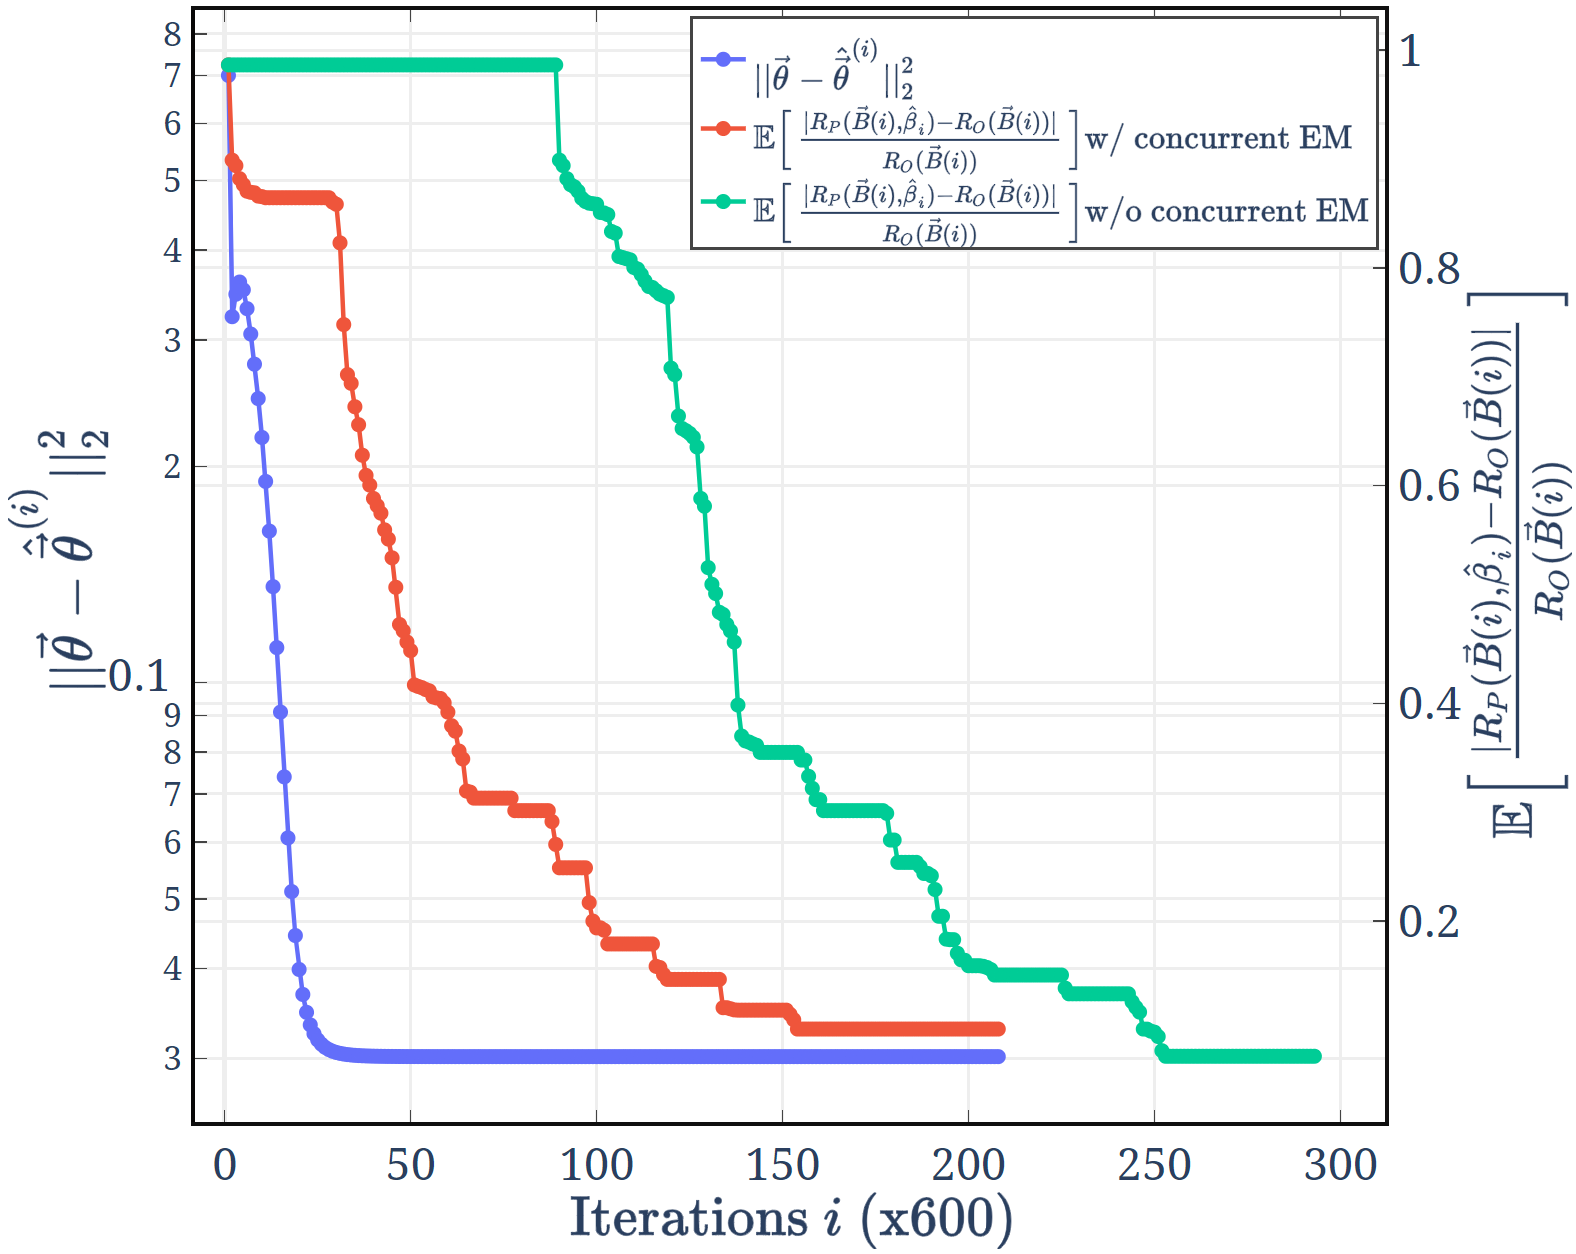
\includegraphics[width = 0.7\textwidth]{figs/Evaluation_1.png}
    \caption{Convergence of: \textcolor{magenta}{MSE of the EM algorithm} to estimate $\vec{\theta}$ $|$ \textcolor{magenta}{Normalized sub-optimality gap} of fragmented PERSEUS with belief update simplification to \textcolor{magenta}{concurrently} find the policy}
    \label{fig:4b}
\end{figure}
\end{frame}
\begin{frame}{Numerical Evaluations (2/2)}
    \begin{figure}
    \centering
    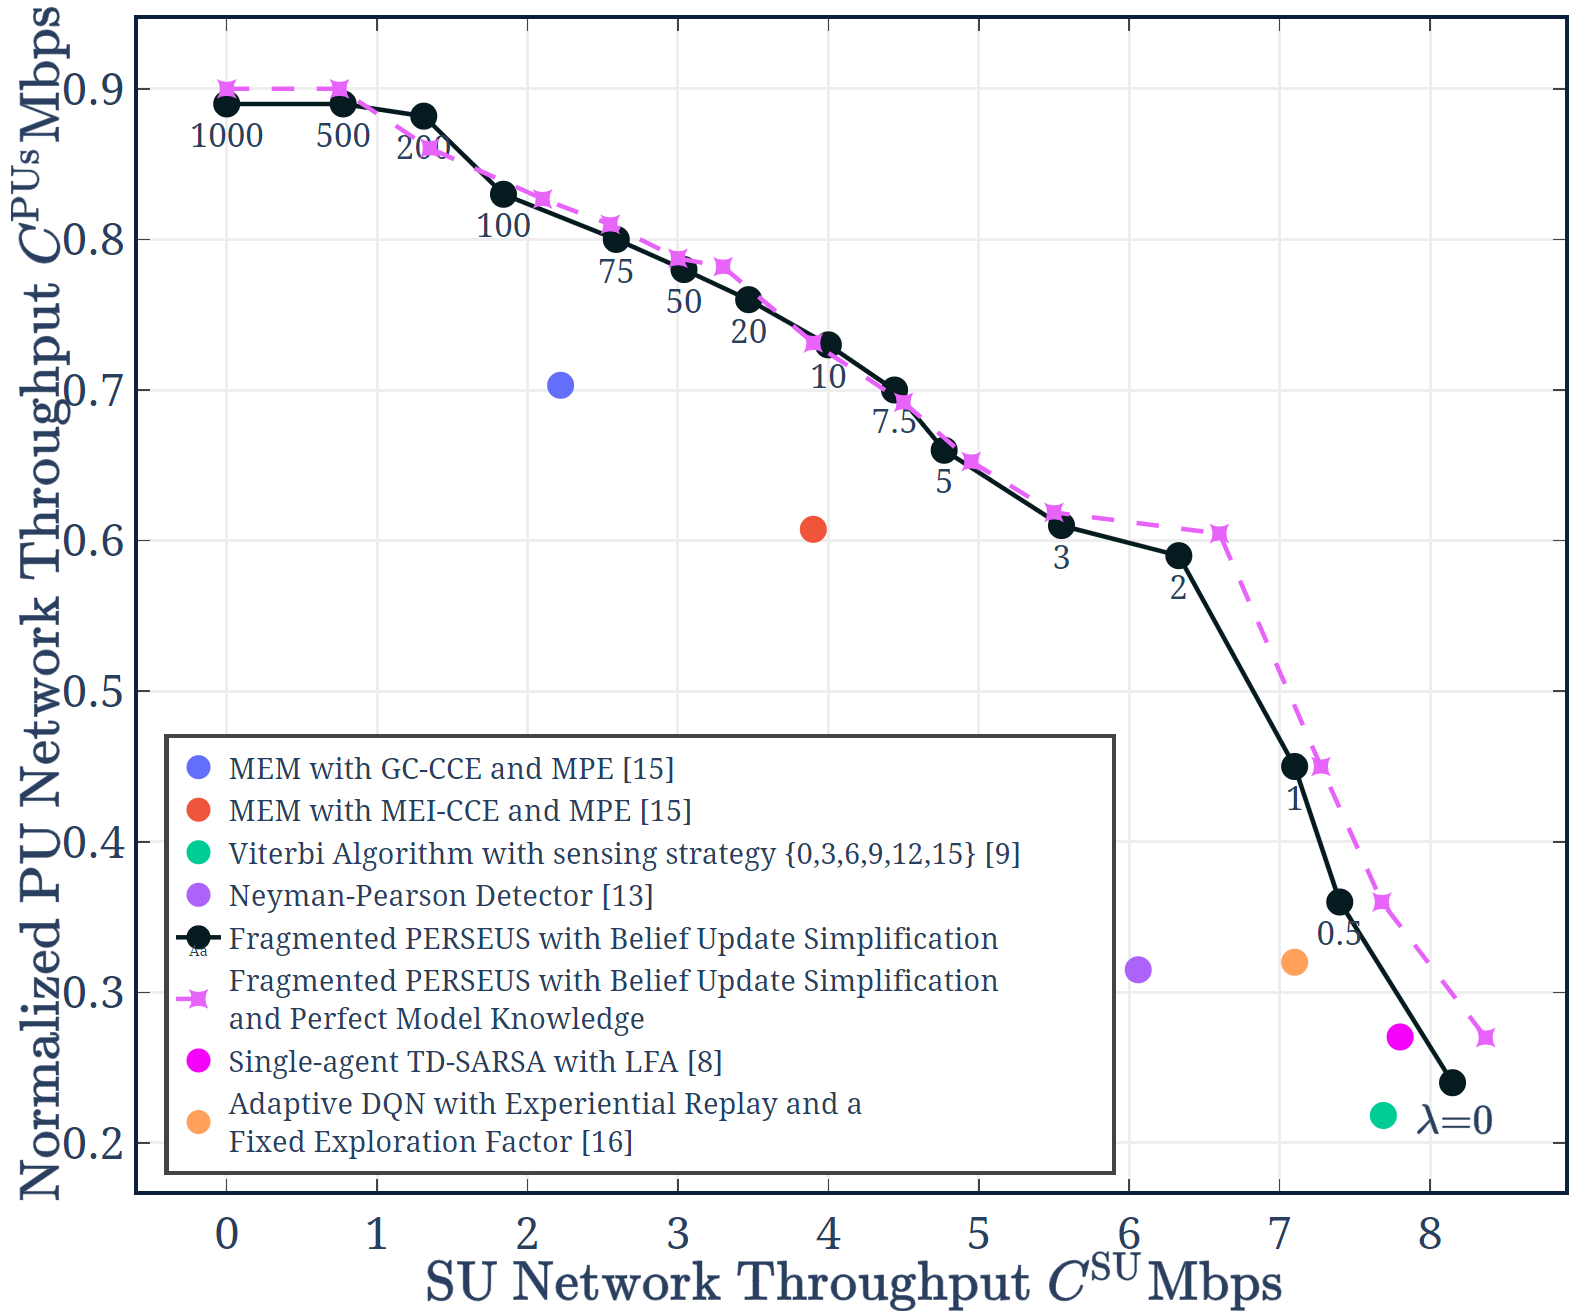
\includegraphics[width = 0.6\textwidth]{figs/Evaluation_2_Reduced.png}
    \caption{$C^{\text{SU}}$ v $C^{\text{PUs}}$ for different values of the penalty term $\lambda$ $|$ \textcolor{magenta}{Comparison with state-of-the-art}}
    \label{fig:4d}
\end{figure}
\tiny{[15]: M. Gao, et. al., ``Fast Spectrum Sensing...", 2014 IEEE MilCom}
\\\tiny{[9]: C. Park, et. al., ``HMM Based Channel Status Predictor for Cognitive Radio", 2007 Asia-Pacific MW Conf}
\\\tiny{[13]: S. Mosleh, et. al., ``Performance analysis of the Neyman-Pearson fusion center...", 2009 IEEE EUROCON}
\\\tiny{[8]: J. Lund\'{e}n, et. al., ``Multiagent Reinforcement Learning...", IEEE Journal of Selected Topics in SigProc, 2013}
\\\tiny{[16]: S. Wang, et. al., ``Deep Reinforcement Learning for Dynamic Multichannel Access...", IEEE TCCN, 2018}
\end{frame}
\begin{frame}{Extensions (1/2): Distributed Multi-agent Deployment\footnote{\tiny{B. Keshavamurthy and N. Michelusi, ``Learning-based Spectrum Sensing in Cognitive Radio Networks via Approximate POMDPs", Under review at IEEE TCCN, 2021}}}
\begin{figure}
    \centering
    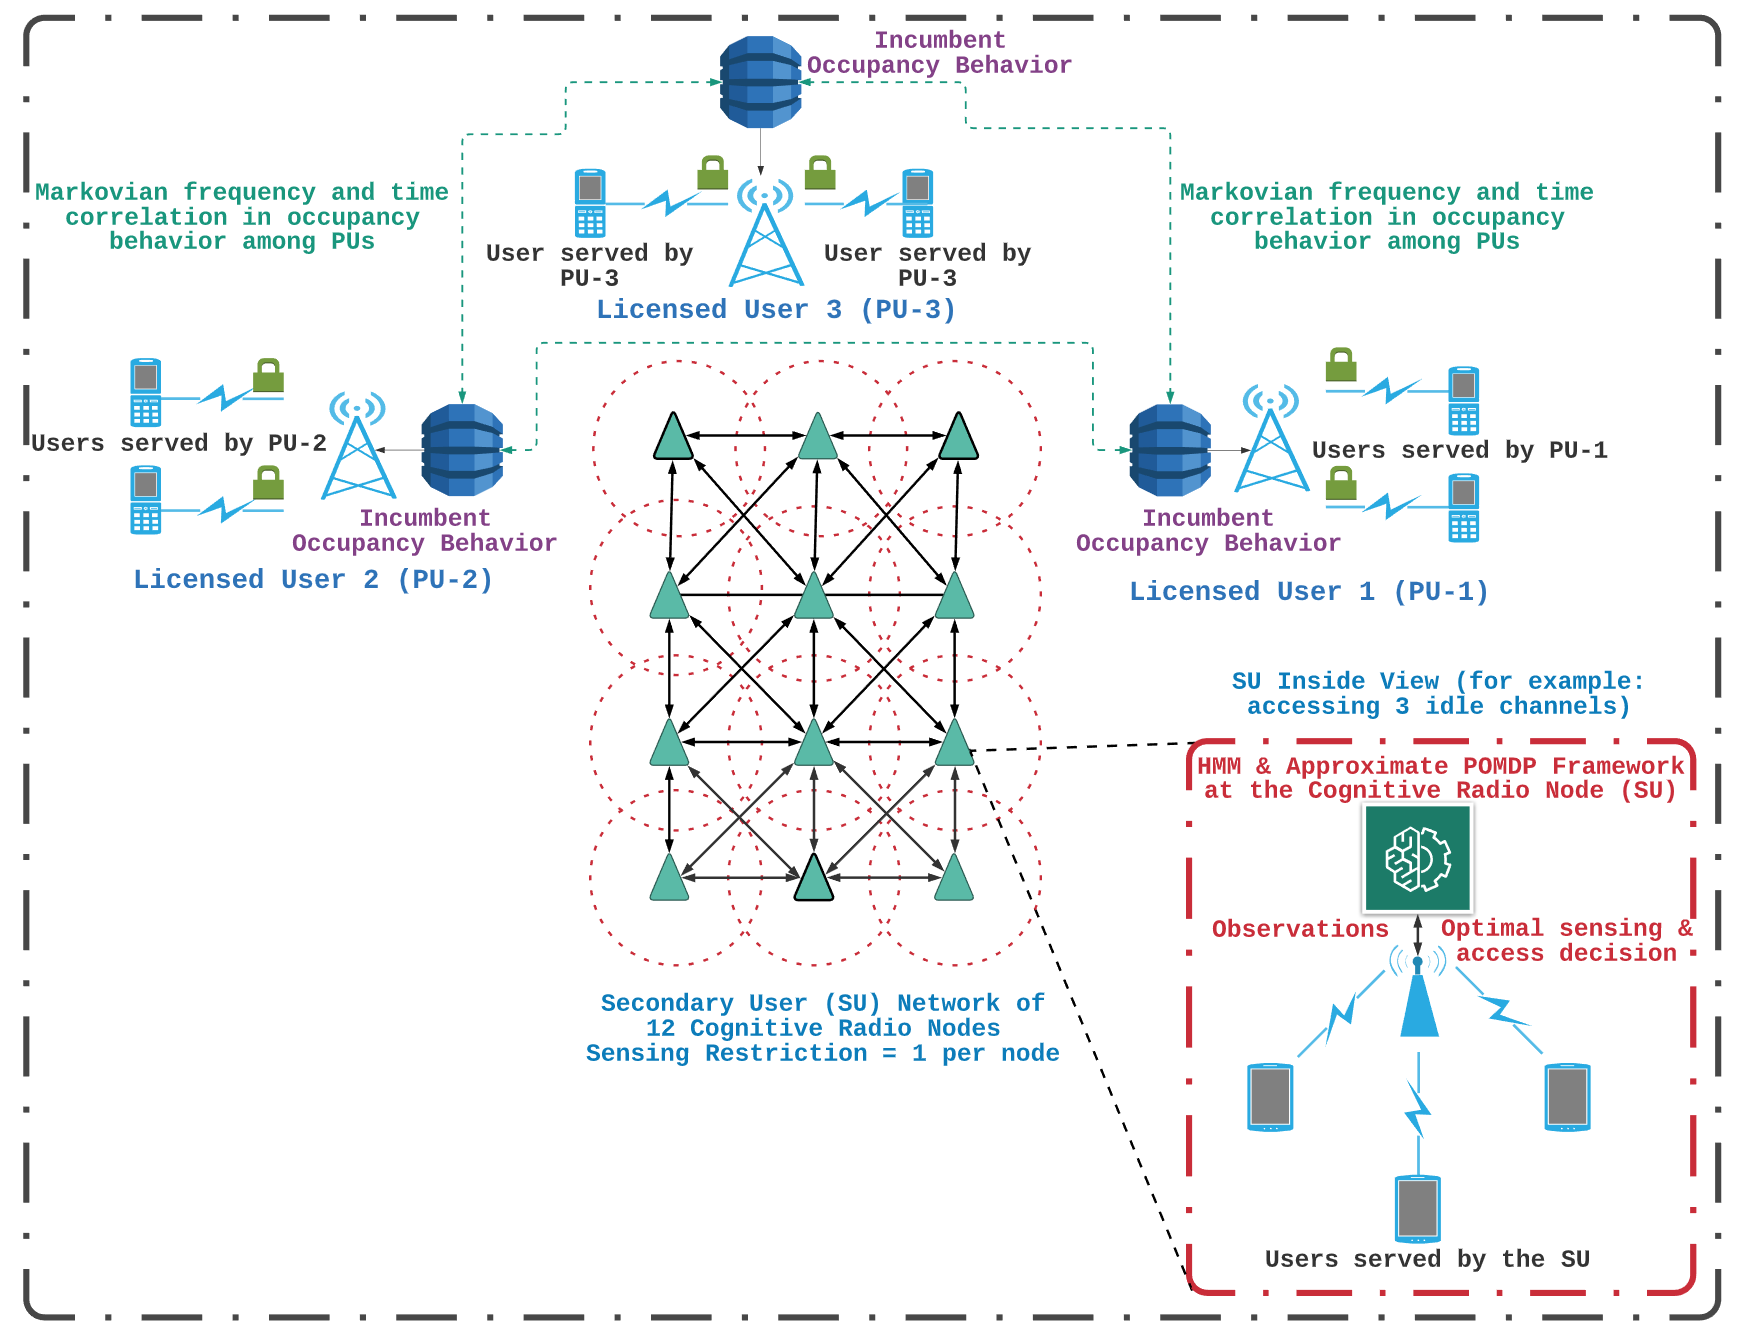
\includegraphics[width = 0.65\textwidth]{figs/Minerva_Multiagent_System_Model.png}
    \caption{Distributed multi-agent example: $18$ channels, $3$ PUs, $12$ SUs}
    \label{fig:5b}
\end{figure}
\vspace{-5mm}
\footnotesize{Also, our multi-agent approximate POMDP solution is evaluated in \textcolor{magenta}{centralized settings} via emulations in the \textcolor{magenta}{DARPA SC$2$ Active Incumbent} scenario\footnote{\tiny{Active Incumbent, DARPA SC$2$, [\href{https://sc2colosseum.freshdesk.com/support/solutions/articles/22000239489-active-incumbent-}{\textcolor{blue}{Online}}], Aug 28, 2019}}.}
\end{frame}
\begin{frame}{Extensions (2/2): Multi-agent POMDP Model\footnote{\tiny{B. Keshavamurthy and N. Michelusi, ``Learning-based Spectrum Sensing in Cognitive Radio Networks via Approximate POMDPs", Under review at IEEE TCCN, 2021}}}
\begin{figure}
    \centering
    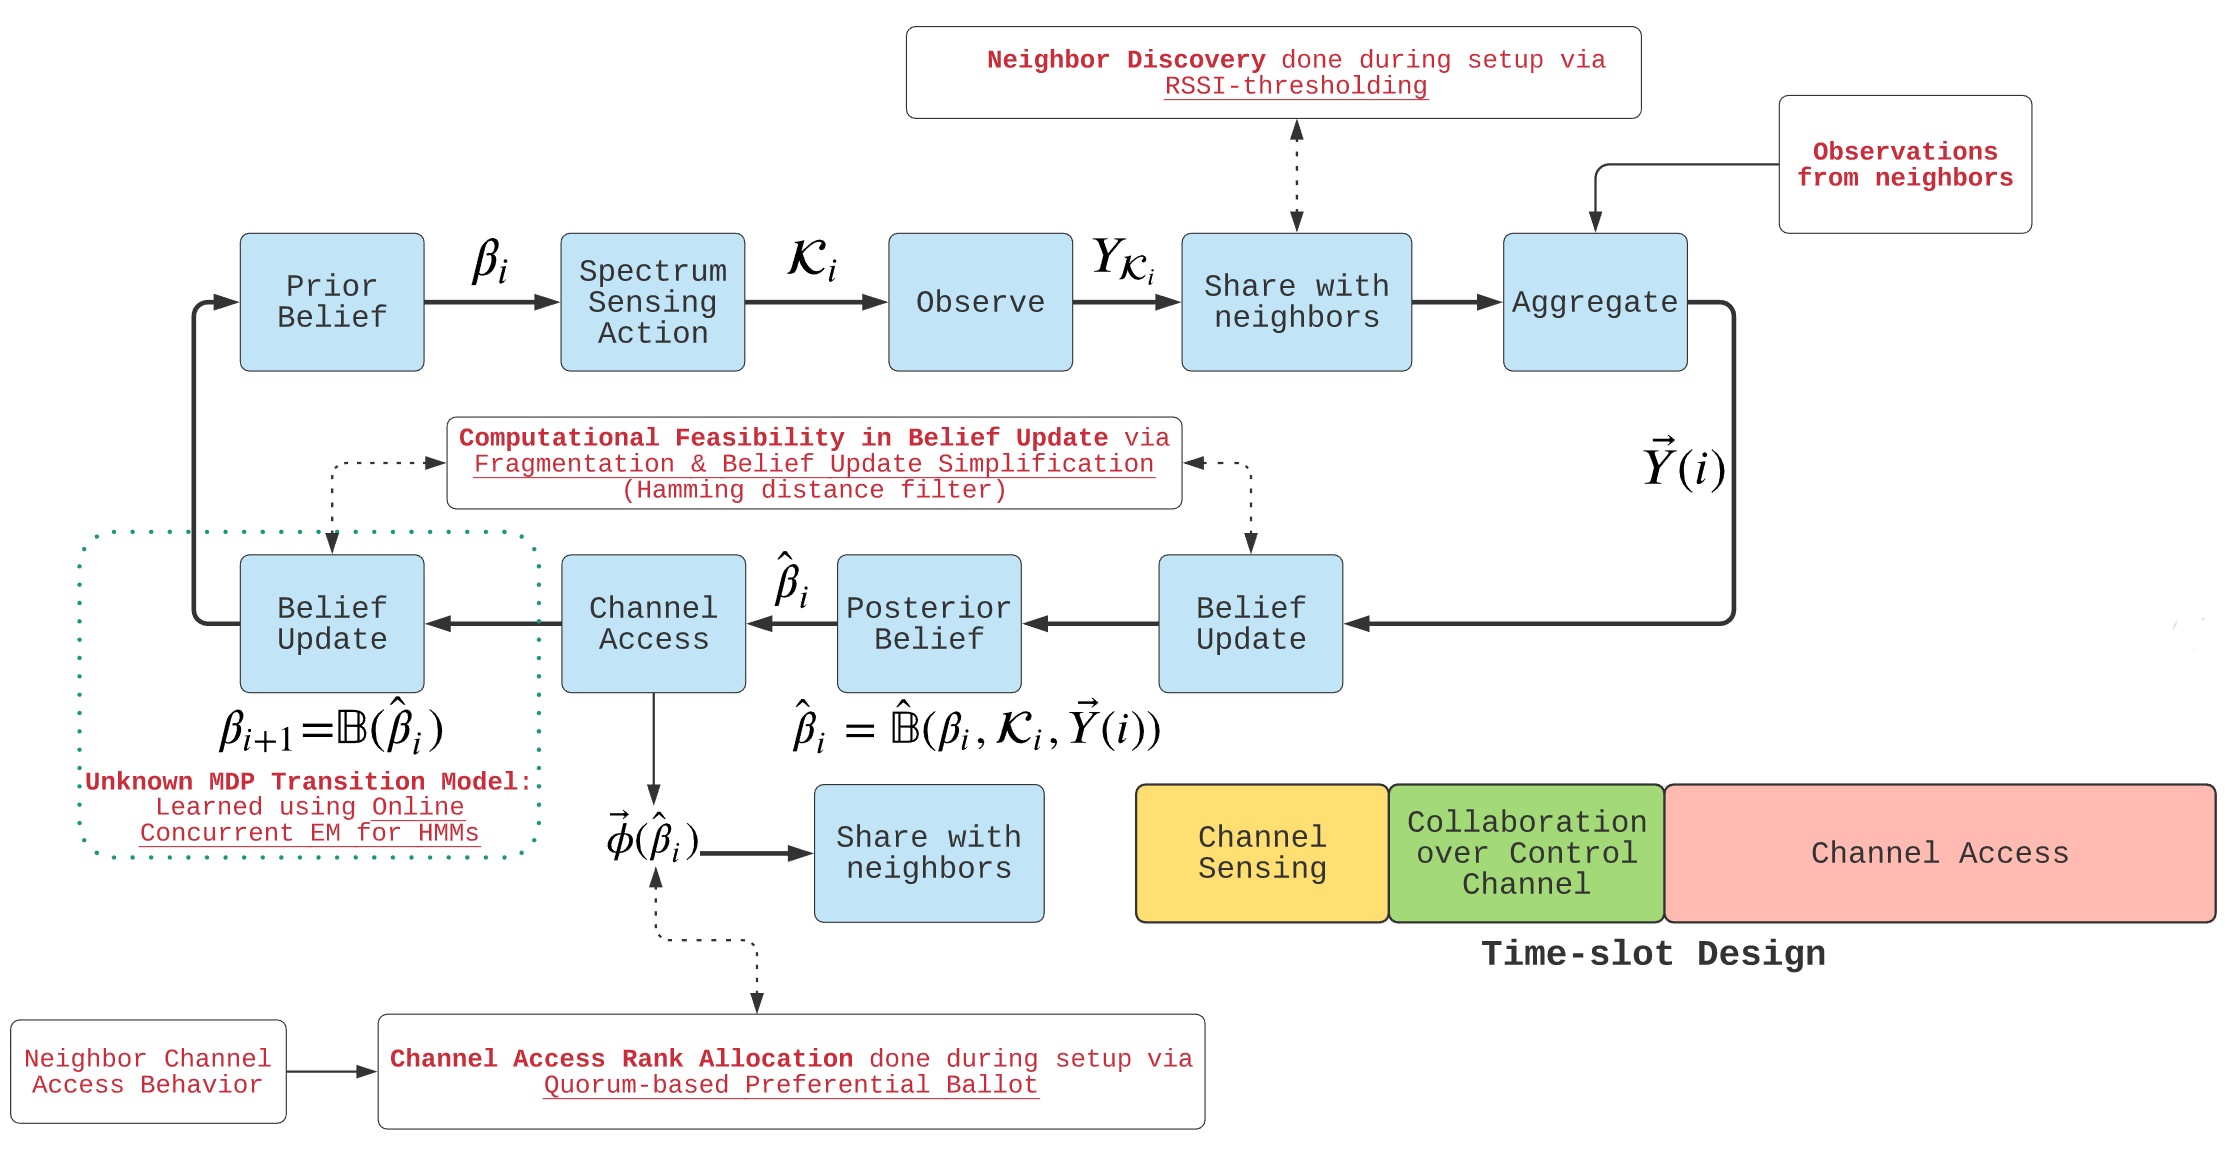
\includegraphics[width = 1.0\textwidth]{figs/POMDP_MultiAgent_Model.PNG}
    \caption{The POMDP model for multi-agent deployments}
    \label{fig:5c}
\end{figure}
\end{frame}
\begin{frame}{Future View}
    \begin{itemize}
        \item \footnotesize{NSF PAWR POWDER\footnote{\tiny{NSF PAWR POWDER, University of Utah, [\href{http://docs.powderwireless.net/}{\textcolor{blue}{Online}}]}} testbed}:
        \begin{itemize}
            \item \footnotesize{\textcolor{magenta}{Over-the-Air (OTA)} [CBRS: $3.4{-}3.8$ GHz] impl of this approximate POMDP solution in multi-agent settings}
        \end{itemize}
    \end{itemize}
    \begin{figure}
        \centering
        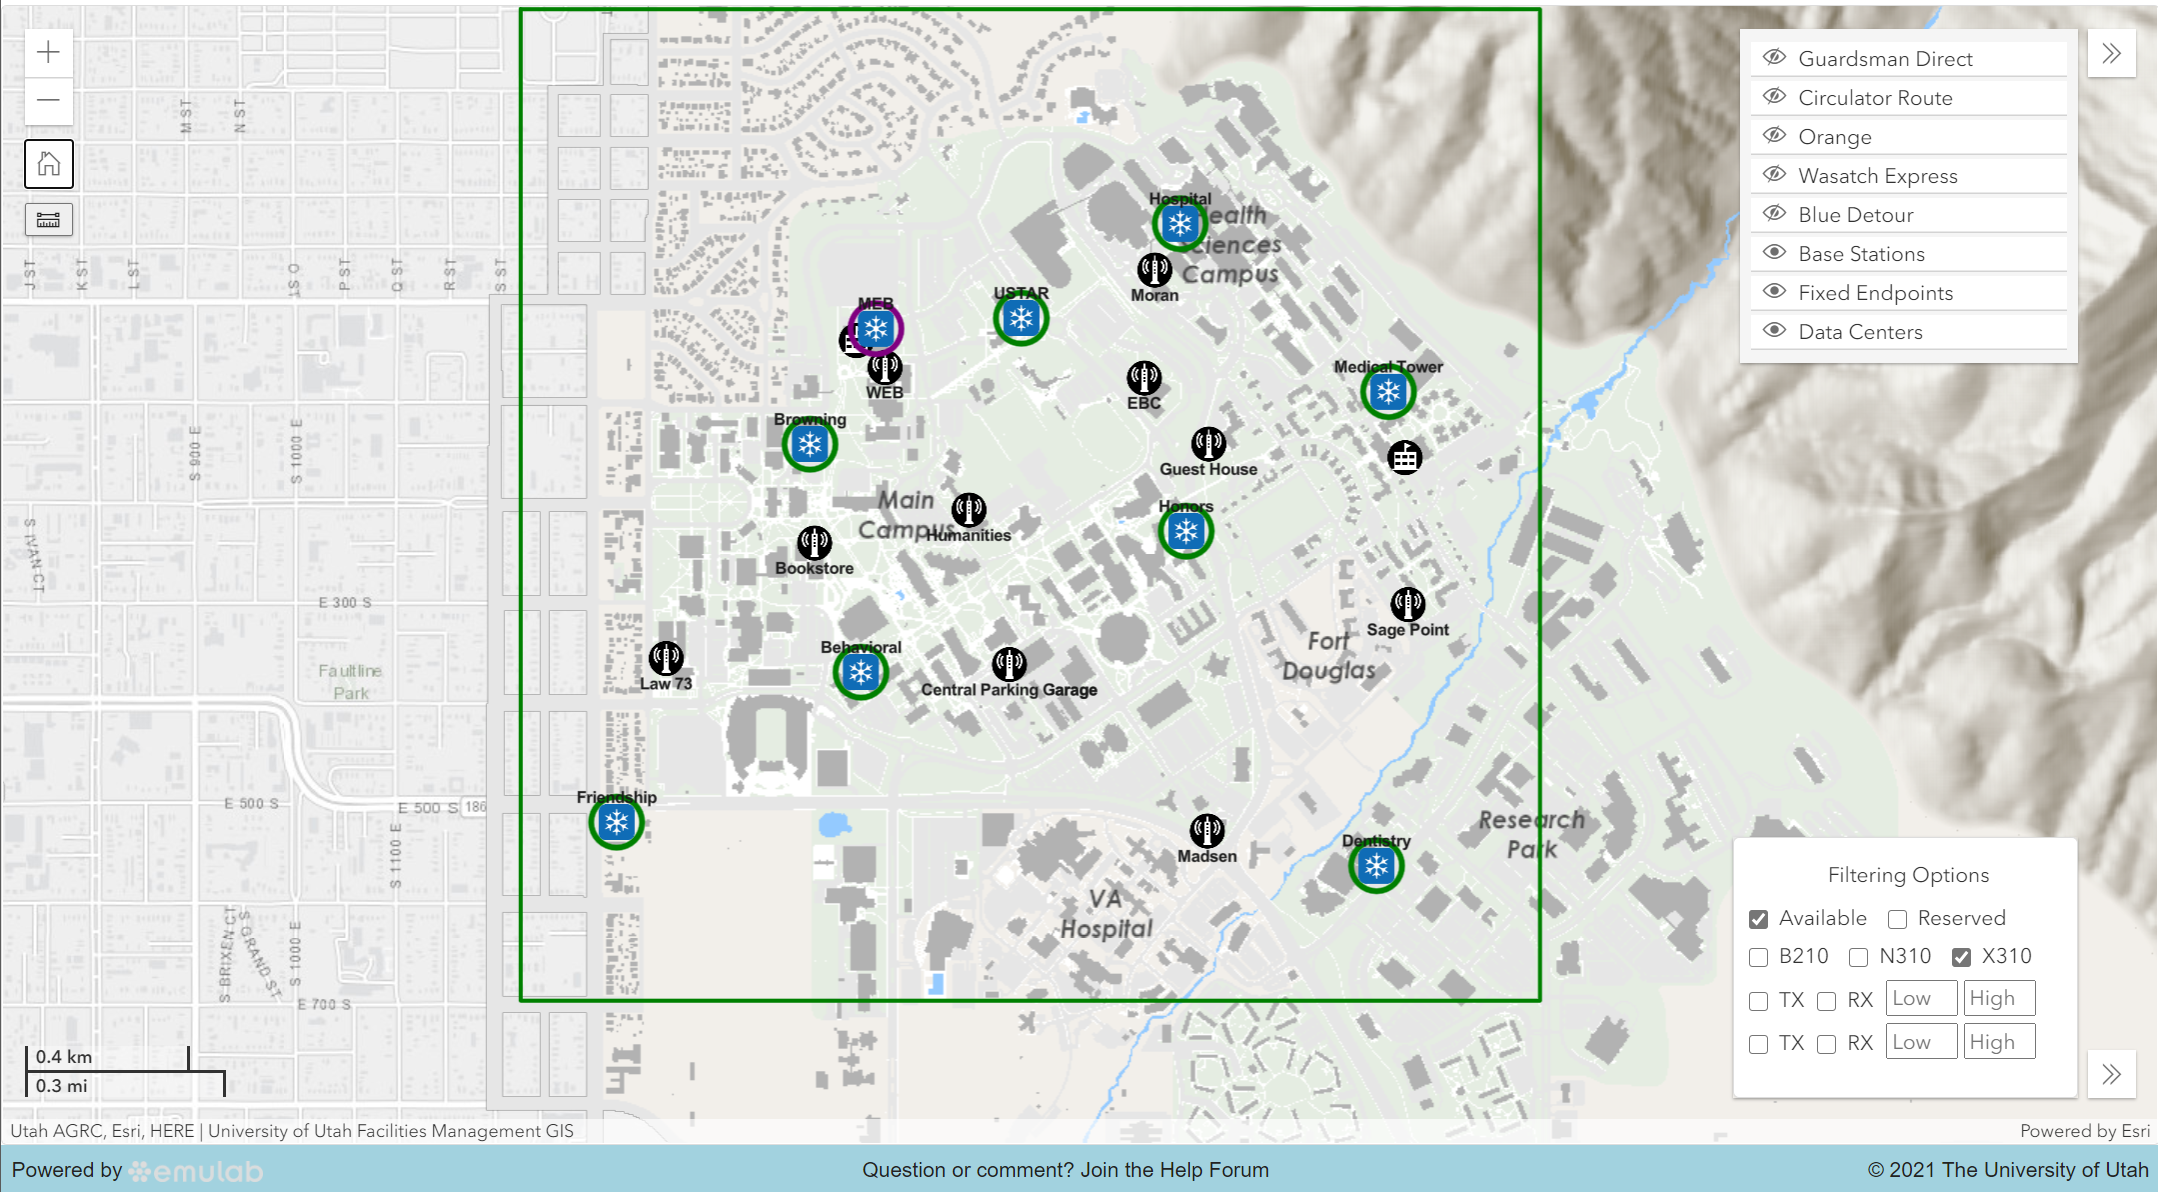
\includegraphics[width = 0.9\textwidth]{figs/POWDER.PNG}
        \caption{POWDER at the University of Utah: our OTA arena}
        \label{fig:5d}
    \end{figure}
\end{frame}
\begin{frame}{Conclusion}
We have \textcolor{blue}{addressed the challenges} \& \textcolor{blue}{proved superior performance:}\\
\begin{itemize}
    \footnotesize{
    \item Time-freq correlated \textcolor{magenta}{PU} occupancies $|$ \textcolor{magenta}{SU} with \textcolor{magenta}{sensing limits}
    \item Fully online \textcolor{magenta}{Baum-Welch} (HMM EM) $|$ Concurrent \textcolor{magenta}{PERSEUS}
    \item \textcolor{magenta}{Fragmentation} $|$ \textcolor{magenta}{Hamming distance state filters}
    \item \textcolor{magenta}{Superior performance} over TD-SARSA, DQN, Viterbi, etc.
    \item \textcolor{magenta}{Regulate the trade-off} between SU and PU throughputs}
\end{itemize}
\end{frame}
\end{document}